\documentclass[aps,pra,twocolumn,notitlepage,superscriptaddress]{revtex4-1}

\usepackage{physics}
\usepackage{xcolor,graphicx}
\usepackage{comment}
\usepackage{siunitx}

\usepackage{amsthm,amssymb}
\usepackage{array}
\usepackage{hyperref}
\usepackage{mathtools}
\usepackage{bm,times,enumitem}
\usepackage{physics}
\usepackage{algorithm}
\usepackage{algc}
\usepackage{algcompatible}
\usepackage{algpseudocode}
\usepackage{soul}
\usepackage{dsfont}

\newcommand{\ns}[1]{\textcolor{magenta}{#1}}

%%
\def \id {\mathds{1}}

\begin{document}

\title{Optimizing quantum-enhanced Bayesian multiparameter estimation in noisy apparata}

\author{Federico Belliardo}
\affiliation{NEST, Scuola Normale Superiore and Istituto Nanoscienze-CNR, I-56126 Pisa, Italy}

\author{Valeria Cimini}
\affiliation{Dipartimento di Fisica, Sapienza Universit\`{a} di Roma, Piazzale Aldo Moro 5, I-00185 Roma, Italy}

\author{Emanuele Polino}
\affiliation{Dipartimento di Fisica, Sapienza Universit\`{a} di Roma, Piazzale Aldo Moro 5, I-00185 Roma, Italy}

\author{Francesco Hoch}
\affiliation{Dipartimento di Fisica, Sapienza Universit\`{a} di Roma, Piazzale Aldo Moro 5, I-00185 Roma, Italy}

\author{Bruno Piccirillo}
\affiliation{Department of Physics ``E. Pancini'', Universit\'a di Napoli ``Federico II'', Complesso Universitario MSA, via Cintia, 80126, Napoli}
\affiliation{INFN, Sez. di Napoli, Complesso Universitario di Monte Sant'Angelo, via Cinthia, 80126 Napoli, Italy}

\author{Nicol\`o Spagnolo}
\affiliation{Dipartimento di Fisica, Sapienza Universit\`{a} di Roma, Piazzale Aldo Moro 5, I-00185 Roma, Italy}

\author{Vittorio Giovannetti}
\email{vittorio.giovannetti@sns.it}
\affiliation{NEST, Scuola Normale Superiore and Istituto Nanoscienze-CNR, I-56126 Pisa, Italy}

\author{Fabio Sciarrino}
\email{fabio.sciarrino@uniroma1.it}
\affiliation{Dipartimento di Fisica, Sapienza Universit\`{a} di Roma, Piazzale Aldo Moro 5, I-00185 Roma, Italy}

\begin{abstract}
Achieving quantum-enhanced performances when measuring unknown quantities requires developing suitable methodologies for practical scenarios, that include noise and the availability of only a limited amount of resources. Here, we report on the optimization of quantum-enhanced Bayesian multiparameter estimation in a scenario where a subset of the parameters describes unavoidable noises in an experimental photonic sensor. We explore how the optimization of the estimation changes depending on which parameters are either of interest or are treated as nuisance ones. Our results show that optimizing the multiparameter approach in noisy apparata represents a significant tool to fully exploit the potential of practical sensors operating beyond the standard quantum limit for broad resources range.

\end{abstract}

\maketitle

The goal of quantum metrology is to estimate a set of physical parameters, exploiting quantum resources to achieve improved performances beyond those achievable by classical methods. The use of quantum probes discloses the capability to reach the Heisenberg limit (HL), gaining a quadratic scaling advantage over the standard quantum limit (SQL) corresponding to the use of $N$ independent probes \cite{Giovannetti1330,PhysRevLett.96.010401,Giovannetti,barbieri2022optical,avsreview2020}. Often in a real scenario, even if the interest relies on a single parameter, the process is unavoidably affected by the presence of unknown noises. For these reasons, it is usually more effective to treat these estimations using a multiparameter approach \cite{liu2019quantum,suzuki2020quantum,suzuki2020nuisance,doi:10.1080/23746149.2016.1230476,albarelli2020perspective}. Despite their importance, experimental demonstrations of quantum enhanced estimation in the multiparameter case are still few and limited to modest amounts of coherent quantum resources \cite{polino2019experimental,liu2021distributed,hong2021quantum,valeri2022experimental,cimini2022deep,avsreview2020}.The following two extremal scenarios are prototypical for multiparameter metrology. In the first case, all the unknown parameters are treated on the same level, and thus one needs to optimize the overall amount of information extracted. Here, the adoption of quantum probes can provide improved performances with respect to strategies where each parameter is estimated separately \cite{humphreys2013quantum,PhysRevLett.128.040504,belliardo2021incompatibility,Yue}. In the second extremal case, only one parameter is considered to be of interest, but the dynamics of the metrological evolution intrinsically involves other nuisance parameters, of which an approximate knowledge is although necessary to retrieve a good estimator for the desired one. For instance, we have to deal with this scenario when different sources of noise affect the evolution: phase and visibility \cite{Roccia:18,roccia2017entangling,cimini2019quantum,cimini2019adaptive}, phase and phase diffusion \cite{Vidrighin,PhysRevLett.106.153603}, magnetic field and decoherence \cite{PhysRevA.84.012103} for example. The optimal strategy in this case is very different from the optimal in the former one, since now the interest is to maximize the information extracted on one parameter at the expense of all the others \cite{goldberg2020multiphase}. In the general case, intermediate configurations between these two extremal scenarios can be defined, corresponding to different choices of the cost function. For example, a couple of parameters could be considered of interest while the others are treated nuisance. For each specific scenario, different strategies may thus turn out to be optimal. In general, the importance of the different parameters can be weighted arbitrarily.

Another crucial aspect for quantum metrology in a practical scenario regards the availability of a finite amount of resources $N$ in the estimation process. The standard approach is based on a theoretical framework that is dedicated to define bounds and strategies in the asymptotic limit of large $N$. However, when only a finite amount of resources is available, any estimation strategy needs to be tailored to optimize the convergence for low values of $N$ \cite{rubio2020quantum,rubio2019limited,rubio2020bayesian}. A powerful tool here is represented by adaptive protocols, which enable faster convergences to the ultimate limits \cite{wiseman1995adaptive,berry2000optimal}. These have been implemented both through online \cite{berni2015ab,Cimini:19} and offline \cite{hentschel2011efficient,lovett2013differential} approaches also resorting to the use of different machine learning algorithms \cite{hentschel2009adaptive,piccoloLume,rambhatla2020adaptive}. These techniques demonstrated two relevant characteristics, namely fast convergence to the ultimate bounds and performances independent of the particular value of the parameter of interest. Different experimental applications of adaptive techniques have been reported, first in single-parameter estimation problems \cite{armen2002adaptive,higgins2007entanglement,daryanoosh2018experimental,wheatley2010adaptive,piccoloLume,rambhatla2020adaptive} and then in a multiparameter setting \cite{Valeri2020}. In this scenario, the versatility of the multiparameter approach allows to choose the optimal allocation of resources, depending on which are the parameters of interest and which are the noises treated instead as nuisances. 

In this work, we investigate a multiparameter estimation scenario, where the parameters of interest are physical rotation angles~\cite{goldberg2018quantum,goldberg2021rotation} together with the noise parameters involved in the interferometric measurements. To this end, we employ orbital angular momentum (OAM) of single photons, carrying tunable OAM values up to $50$, able to show N00N-like sensitivities for rotation estimations \cite{dambrosio_gear2013,cimini2021non,Fickler13642,barnett2006resolution,jha2011supersensitive,PhysRevLett.127.263601}. Importantly, we extend the single parameter study \cite{cimini2021non} to a multiparameter approach within a Bayesian framework \cite{helstrom1976quantum,box2011bayesian,d2022experimental,rubio2020bayesian} for all the aforementioned scenarios by employing an adaptive strategy ensuring the optimal allocation of resources \cite{granade2012robust}. Such approach allows us to extend the multiparameter estimation problems to the regime of $O(30,000)$ number of quantum-like resources, experimentally demonstrating sub-SQL precision in the estimation of the rotation angle for wide resources ranges even with nuisance parameters. In order to quantify the quality of the reached performances, we define non-tight Bayesian bounds on the estimations in each considered scenario.

\emph{Precision bounds-}
%
The goal of multiparameter quantum metrology is to identify regimes where the estimation precision outperforms the one achievable by classical probes. A crucial aspect is to keep such enhanced performances as the employed resources increase. It becomes key to develop a platform able to investigate such regime with quantum scaling of the precision. Here, we study the contemporary estimation, in the large resource regime, of a rotation angle $\theta\in [0,\pi)$ and of a collection of parameters (the fringe visibilities $V_{s_1}$, $\cdots$, $V_{s_4}$ defined below) that affect the efficiency of the detection process~\cite{dambrosio_gear2013}. More specifically, in our scheme, before each measurement step we preselect a control parameter $s$ out of a set of four possible values $\{s_1=1,s_2=2,s_3=11,s_4=51\}$. In the ideal (noiseless) scenario such choice is meant to force the interferometer to produce a single-photon, N00N-like output state analogous to those employed in \cite{higgins2007entanglement} to achieve quantum limited precision, i.e. the vector $|\psi_s(\theta)\rangle:=\frac{1}{\sqrt{2}} (\ket{0}+e^{-2is\theta}\ket{1})$, with $|0\rangle$, $|1\rangle$ being orthogonal circular polarization states. Unfortunately, the selection of $s$ also has the indirect effect to add noise into the model which ultimately deteriorate the visibility of the measurements we perform on $|\psi_s(\theta)\rangle$ to recover $\theta$: our scheme relays on two different types of detections, the first corresponding to the projection of $|\psi_s(\theta)\rangle$ on the basis $\{ (\ket{0}\pm \ket{1})/\sqrt{2}\}$, while the second uses $\{ (\ket{0}\pm i \ket{1})/\sqrt{2}\}$ as reference basis: in both cases the choice of $s$ will decrease the visibility to same value $V_s\in[0,1]$, that one could determine from the measured data. Our interest lies in determining how the estimation precision changes depending on the different perspective from which the multiparameter problem is addressed. To this end, we apply the Bayesian algorithm in Ref.~\cite{granade2012robust}, with some minor modifications to account for the circular nature of the rotation angle. This procedure identifies the most effective adaptive strategy depending on the different roles assigned to each parameter (i.e. $\theta$, $V_{s_1}$, $V_{s_2}$, $V_{s_3}$, and $V_{s_4}$), whether they are of interest or are treated as nuisance parameters. In this protocol, the Bayesian posterior probability distribution for all the parameters is represented by a particle filter. From the information accumulated in it, at each step, a greedy strategy selects the experimental settings that minimizes the future expected weighted sum of the estimator variances \cite{granade2012robust}. In our case, we select both the value $s$ that determines the successive probe state and which basis for the polarization measurement we are supposed to use for the measurements of the associated output state $|\psi_s(\theta)\rangle$. These are the controls that the Bayesian procedure for experimental design will optimize. To quantify the efficiency of the estimation, we define a suitable figure of merit and derive bounds limiting its minimal achievable value for the investigated metrological task. For this purpose given $N\gg 1$ integer, we focus on a generic experimental run ${{\mathbf r}_N}$ composed by series of individual measurements where, given $i\in \{1,\cdots, 4\}$, the control value $s_i$ is used $\nu_i$ times, and it is selected under the global constraint $N =\sum_{i=1}^4 \nu_i s_i$ (this is the total number of ``black-box'' resources~\cite{PhysRevLett.96.010401} we dedicate to the recovering of the parameters, with our N00N-like states, see \cite{SI} for details). More precisely, ${{\mathbf r}_N}$ is a string of containing the list of $s$, the polarization basis chosen for each photon and the outcome of each measurement, see the Supplementary Information~\cite{SI} for more details. Indicating hence with $\hat{\theta}^{({\mathbf r}_N)}, \hat{V}^{({\mathbf r}_N)}_{s_1}, \cdots, \hat{V}^{({\mathbf r}_N)}_{s_4}$ the estimate values of ${\theta}, {V}_{s_1}, \cdots, {V}_{s_4}$ we get from the procedure, we gauge the associated error via the quantity $\Delta^{2}_{{\mathbf r}_N,G}(\theta):=G_{1,1}|\hat{\theta}^{({\mathbf r}_N)}-\theta|^2 + \sum_{i=1}^4 G_{i+1\, , i+1} |\hat{V}^{({\mathbf r}_N)}_{s_i}-V_{s_i}|^2$, where $G$ is a weight matrix that controls which parameters are to be treated as nuisance and which are the parameters of interest~\cite{goldberg2020multiphase}. To remove accidental dependence upon the explicit value of $\theta$ or on the specific choice of ${{\mathbf r}_N}$, we repeat the whole estimation for a random collection $\theta_1, \theta_2,\cdots,\theta_J$ of $J$ different values of $\theta$, and for each $\theta_j$, run the whole procedure $M$ times. In our $J=8$ and $M$ was at least $200$ for each angle. This finally leads us to the identification of the following figure of merit,
%
\begin{equation}
\mathcal{M}^2_G := \text{Median} \Big[ \frac{1}{J}
	\sum_{j=1}^J \Delta^{2}_{{\mathbf r}_N,G}(\theta_j) \Big] \; ,
	\label{eq:medianMerit}
\end{equation}
%
which we express in terms of the median instead of the expectation value on the Bayesian posterior distribution, due to the fact that the former is much less sensitive to outliers that are always present in the task of rotation estimation~\cite{cimini2021non}. It is possible to impose a theoretical lower limit on~(\ref{eq:medianMerit}) which can be used to evaluate the quality of our experimental data. Specifically, we can write
%
\begin{equation}
	\mathcal{M}^2_G \gtrapprox \xi {C_G}/{N} \; ,
	\label{eq:boundMSE}
\end{equation}
%
with $C_G$ being a constant determined by solving numerically an optimization for the Mean Square Error (MSE) of the estimation, and $\xi$ a pre-factor that helps in translating the MSE bound into an inequality for the median error~\cite{SI}. Experimentally, we observe that the value of the visibility depends on the phase $\theta$, although this is a small effect. We have taken that into account by inserting in $\Delta_{{\boldsymbol{r}_N}, G}^2 (\theta_j)$ the actual value of the $V_{s_i}$.

\emph{Experimental apparatus -}
%
In order to investigate a multiparameter metrological problem, we employ a state-of-the-art experimental apparatus, that allows to generate single-photon high-OAM value states showing quantum-like sensitivities for the estimation of a rotation angle. Importantly, we extend the result from the single parameter case \cite{cimini2021non} to a multiparameter one, exploring unprecedented regimes for multiparameter quantum metrology. The experimental setup is composed of a series of q-plates \cite{marrucci-2006spin-to-orbital,cimini2021non} with an increasing topological charge $q$ arranged in a cascade configuration as reported in Fig.~\ref{fig:setup}. Starting from single photons prepared in the horizontal polarization state, we can generate a N00N-like state in the OAM degree of freedom of the form: $\frac{1}{\sqrt{2}}(\ket{0}\ket{m}+\ket{1}\ket{-m})$, where $\ket{0,1}$ refers to the circular polarization, while $\ket{\pm m}$ with $m=2q$ represents the OAM state and depends on the activated q-plate. The prepared state is then sent to a measurement stage composed of the same set of q-plates in reverse order, allowing to reconvert the OAM state into a polarization state. Such measurement stage can be rotated by an angle $\theta\in[0, \pi)$ by means of a fully motorized rotation cage, as realized in Ref. \cite{cimini2021non}. In this way, the photon state passing through the full setup becomes the vector $|\psi_s(\theta)\rangle$ defined earlier, where $s=2q+1$ is the total angular momentum of the photon. By appropriately choosing the active q-plate, the imparted value of $m$ changes, giving the possibility to tune the frequency of the oscillation interference fringes. Finally, through a half-waveplate after the q-plate, it is possible to select also the measurement polarization basis. As anticipated, we can perform our measurements either in the horizontal/vertical polarization basis or in the diagonal one. Given the employed devices, we have access to states with $s = 1,2,11,51$. The first is obtained when no q-plate is activated, while the others are achieved activating in turn one and only one of the three mounted q-plates in the preparation stage, and the corresponding one in the receiver. These states generate oscillation patterns, retrieved from measurements in the polarization basis and characterized by visibilities $V_s$ which depend upon the selected $s$.
%
\begin{figure}[!t]
	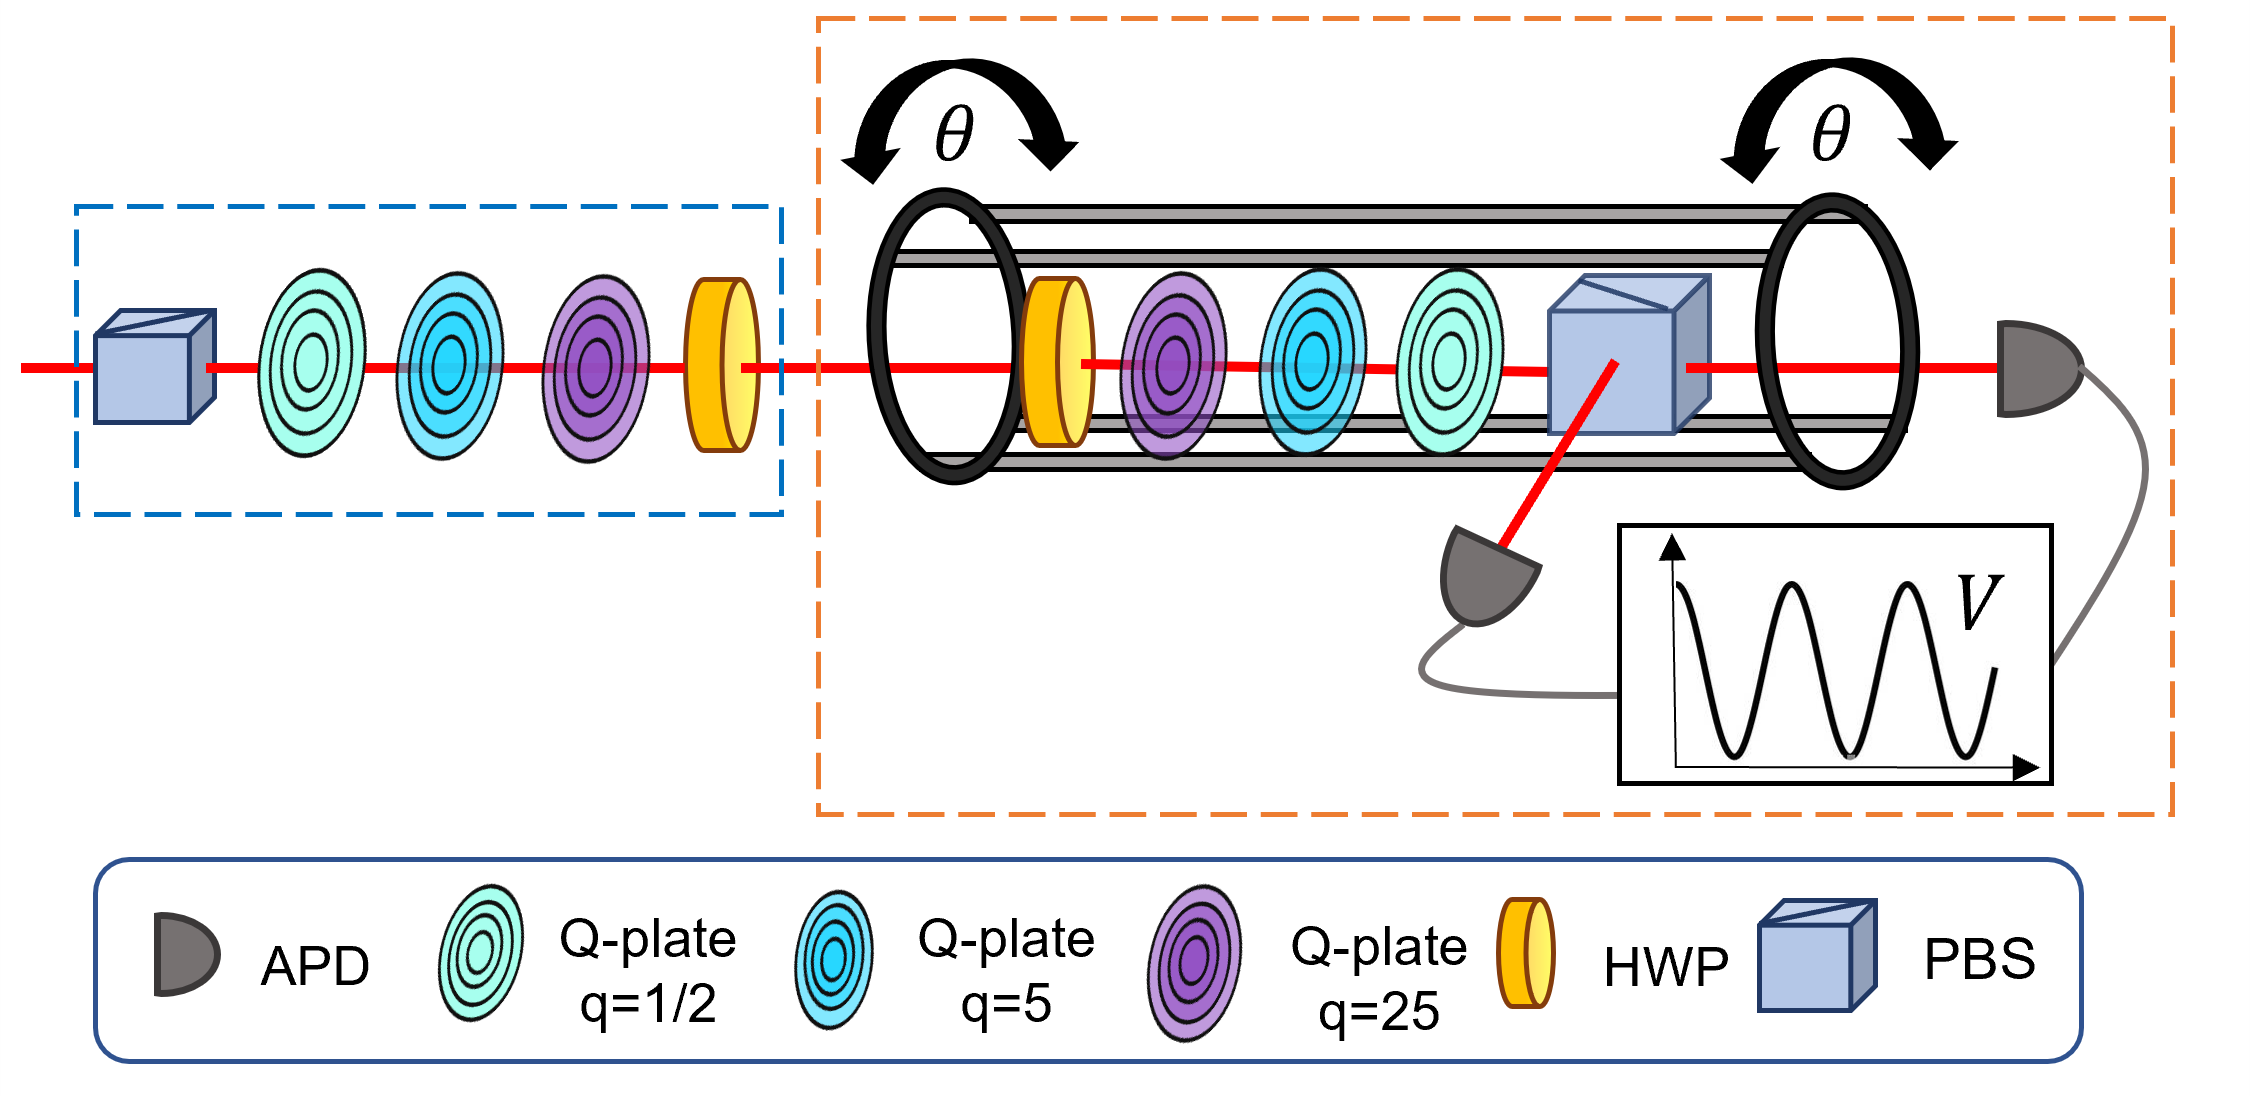
\includegraphics[width=0.99\columnwidth]{setup.png}
	\caption{Sketch of the experimental setup. Single photons are sent through the apparatus consisting of a generation stage (blue rectangle) and a measurement stage (orange rectangle). The first is composed by a polarizing beam splitter (PBS) and three q-plates with different topological charges $q = 1/2; 5; 25$, respectively, followed by a half-waveplate (HWP).
	 The measurement stage is composed by the same elements of the preparation mounted in a compact and motorized cage which can be rotated by an angle $\theta$. After the final PBS, the photons are measured through avalanche photodiodes (APDs). The measurement HWP allows to set the polarization measurement basis.}
	\label{fig:setup}
\end{figure}
%

\emph{Results and discussion -}
%
We start measuring the angle $\theta$ while treating the visibilities as nuisance unavoidable noises. To this end, we set the weight matrix $G$ in Eq.~\eqref{eq:medianMerit} to have $G_{11} = 1$ as the only non-null entry. The data analysis is performed offline, and the raw data contains the outcome of the polarization measurement at the end of the receiving apparatus for many photons, for each rotation angle, q-plate, and polarization basis considered. We perform such measurements for $J=8$ different rotation angles in~$[0, \pi)$. On such collected measurement results we perform the Bayesian analysis setting the prior distributions on the visibilities as uniform in $[0, 1]$, like the prior on the angle which is uniform in $[0, \pi)$. With the objective of minimizing the median error on the estimation of the rotation angle, the adaptive algorithm selects at each step the most appropriate quantum-like resource among the available ones. From the insert of Fig.~\ref{fig:phase}a it can be inferred, that the estimation precision on the rotation angle is optimized by increasing gradually the momentum of the generated OAM states. The precision figure of merit achieved with such optimization strategy is reported in the main plot of Fig.~\ref{fig:phase}a, where the experimental data are compared with the bound on the median in Eq~\eqref{eq:boundMSE}, the Standard Quantum Limit (SQL) error $1/N$ and the ultimate Heisenberg limit (HL) $\pi/N^2$~\cite{PhysRevLett.124.030501}. The (asymmetric) confidence interval for the median (in light red) is evaluated with a bootstrap procedure for a $99\%$ confidence level. The experimental results show that the obtained error approaches the computed bound, which has proved to be a valid reference even if non-tight. Notably, in such scenario, even if the visibility values are completely unknown, the implemented multiparameter protocol shows an enhanced estimation precision compared to the SQL in a large resources range, previously unexplored by multiparameter estimation experiments. Importantly, differently from \cite{cimini2021non} where the measurement strategy has been precalibrated according to the visibility values, here we show that it is still possible to obtain a non-negligible region showing a Heisenberg scaling precision treating the $4$ visibilities as nuisance parameters. 
%
\begin{figure*}[!htb]
	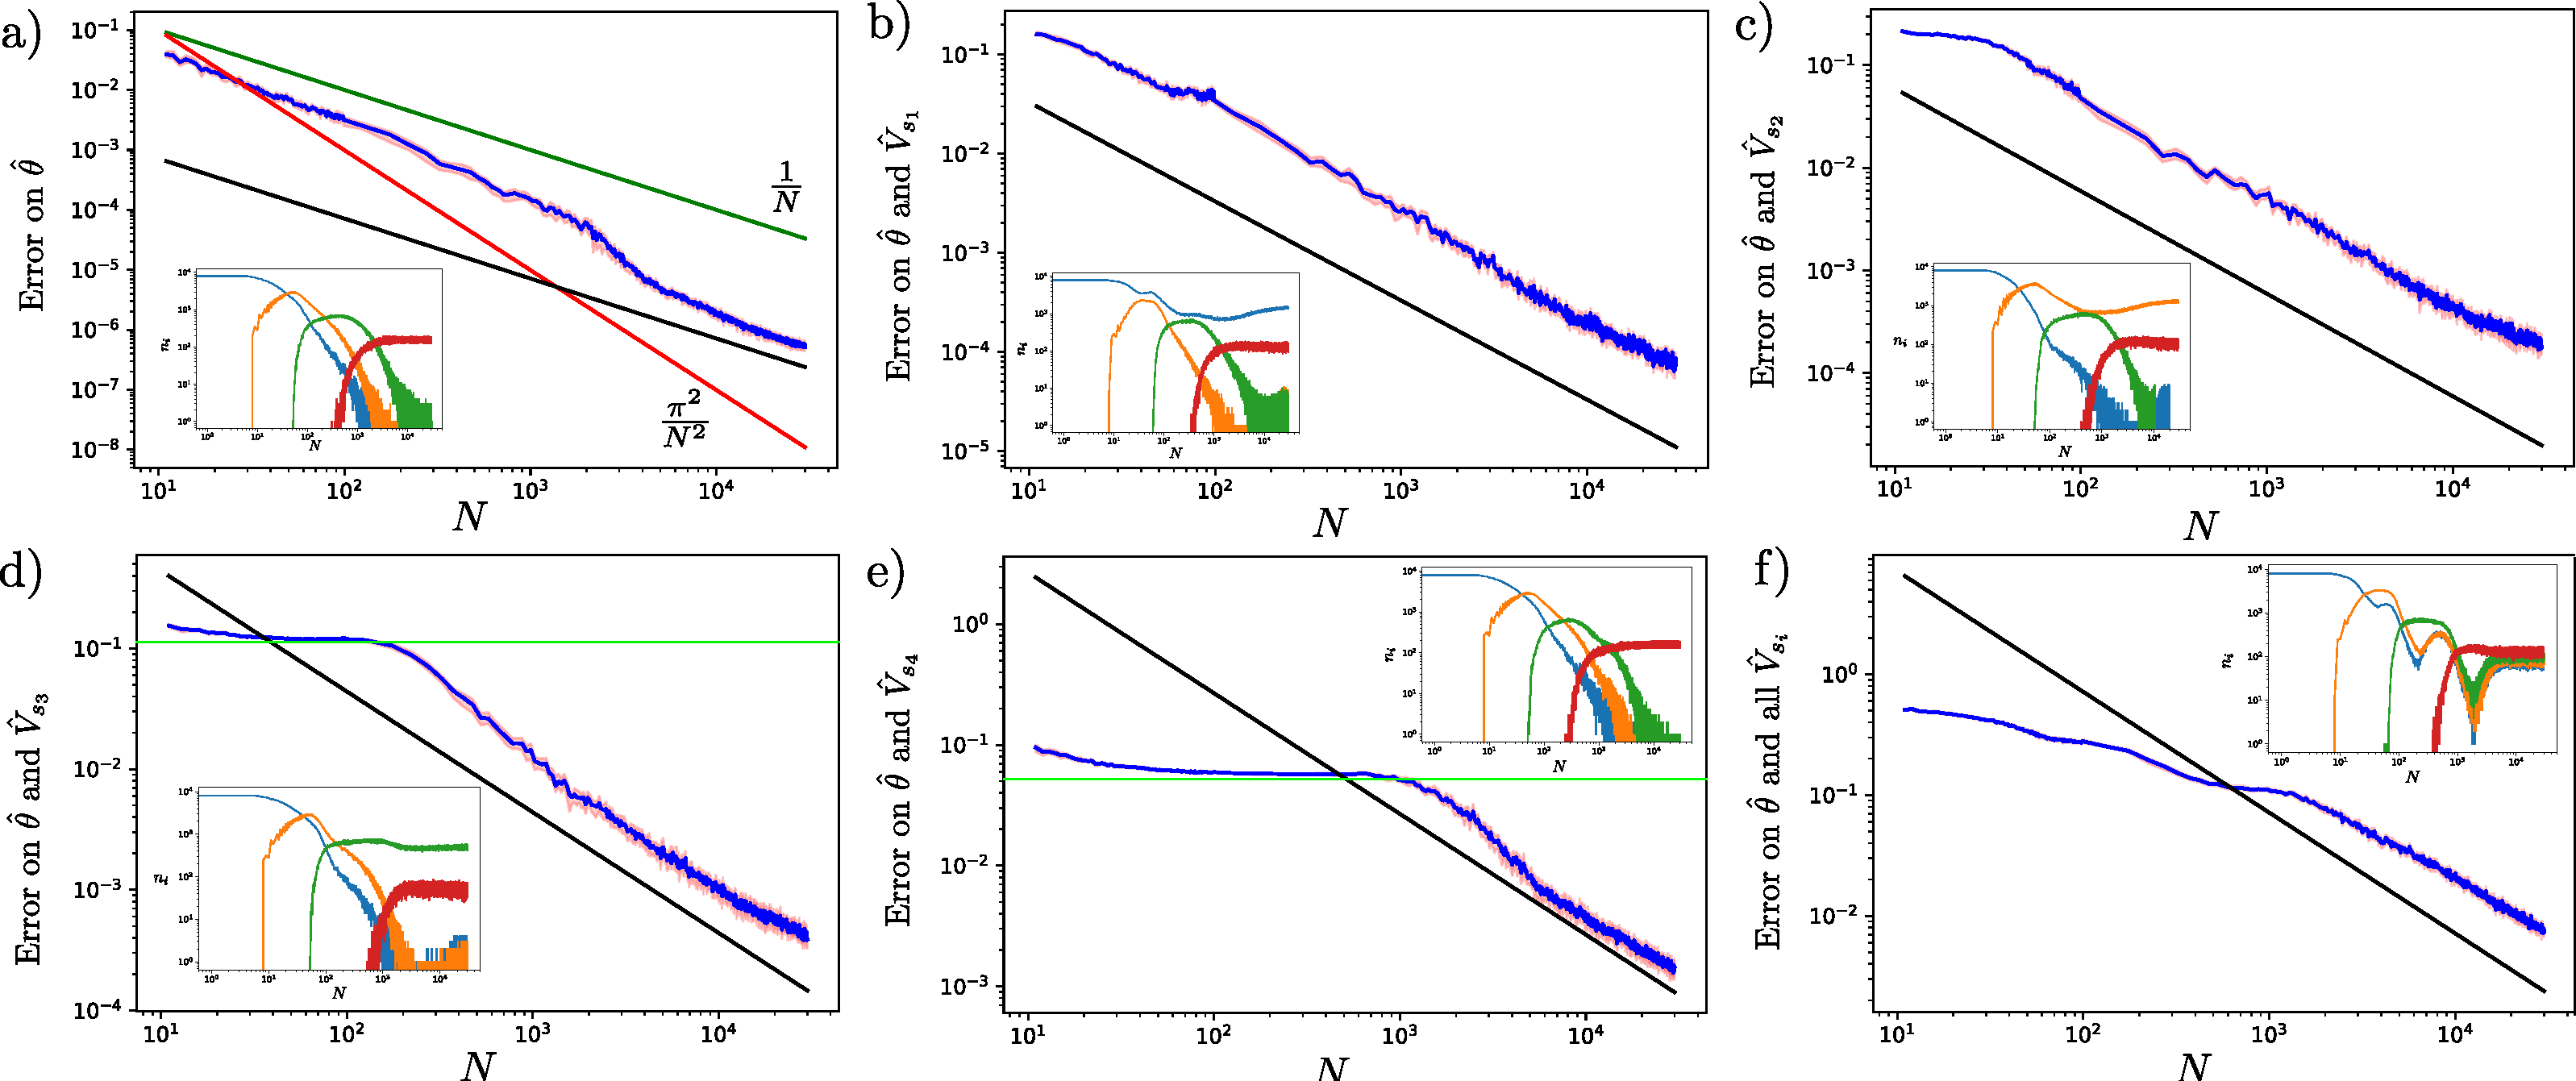
\includegraphics[width=\textwidth]{precision_and_inserts.pdf}
	\caption{a) Plot of the median error for the phase only, with all the other parameters treated as nuisance parameters. The green line is the SQL$=1/N$, and the red one the HL$=\pi^2/N^2$. For all the plots the inserts are the number of uses of each q-plate in a batch of $10^3$ experiments for each of the $J=8$ angles as a function of the number of resources. In the inserts the blue lines correspond to photons with no OAM, the orange lines to $s=2$, the green lines to $s=11$ and the red ones to $s=51$. The intersection of these lines corresponds to the point at which the algorithm starts to suggest a q-plate with higher topological charge to perform the next experiment. Plots b), c), d), and e) refer respectively to the joint median error of the phase and each visibility $V_{s_1}$, $V_{s_2}$, $V_{s_3}$ and $V_{s_4}$. For each plot, all the other three visibilities are treated as nuisance parameters. Plot f) represent the precision for the phase and the joint estimation of all the visibilities. The green lines in d) and e) highlight the plateaus in the precision, that are discussed in the main text. The d) and e) plots show a scaling that in a limited region outperforms the classical ones, (which is the slope of the black line). In all plots, the black line is the RHS of Eq.~\eqref{eq:boundMSE} computed for the appropriate weight matrix $G$, that is the bound on the median.}
	\label{fig:phase}
\end{figure*}
%

Then, we face the scenario where the visibilities are not treated anymore as nuisances but become themselves parameters which have to be estimated. This happens for instance if the user is interested in the full characterization of an interferometer, and therefore needs an estimation of the noise level too. It is interesting to see how the optimization of the available resources changes in these new configurations. In particular, we shall focus on the scenario where one is interested in the estimation of the rotation angle and one of the visibilities (say the $i_0$-th one), while the remaining ones are still treated as nuisance parameters. Under this assumption, the parameters of interest are the pair $(\theta, V_{s_{i_0}})$ with an associated median~(\ref{eq:medianMerit}) computed by taking $G_{1,1}=G_{i_0,i_0}=1$ as the only non-zero elements of $G$. As shown in Fig.~\ref{fig:phase}, under this circumstance the Bayesian protocol, although switching to higher dimensional OAM states to decrease the error on the rotation angle, continues to use the q-plate related to the visibility chosen: this is necessary to obtain a good precision on the joint error. The results of the estimation of each of the four possible couples are reported in Fig.~\ref{fig:phase}b, c, d and e. In particular, the plateau in Fig.~\ref{fig:phase}d and Fig.~\ref{fig:phase}e appear since, for few resources, the q-plates corresponding to $s=11$ and $s=51$ are not significantly used. Therefore, the estimator of the corresponding visibilities remains the mean value of the uniform distribution in $[0, 1]$ (the prior), i.e. $0.5$, while the error on the phase decreases, thereby reaching a plateau determined by the value of the visibility $V_{i_0}$ itself. This changes only when the algorithm starts to use the high charge q-plates, and the error finally decreases.
%
As a final observation we notice that in the case where one focuses only on the phase $\theta$ there is still a pretty large region in which the slope of the estimation error approaches the HL scaling (specifically looking at Fig.~\ref{fig:phase}a), this happens for values of $N$ between 2000 and 5000). Such behavior on the contrary is depressed when considering the estimation of the coupes $(\theta, V_{s_{i_0}})$ (only for $i_0=4$ there is a clear reminiscence of this, see Fig.~\ref{fig:phase}e)). The reason for such behavior has to do with the fact that the visibility is an inherently classical parameter and cannot benefit from the high angular momenta that represent our quantum resources. The enhanced precision on the phase is however retained in the joint error $\mathcal{M}^2_G$ in the estimation, only that it is not noticeable when confronted with the precision on $V_{s_{i_0}}$, except for $s=51$.

In summary, quantum sensing promises to be one of the first quantum technologies exploited to enhance tasks with respect to what is achievable with classical resources. Most of the realistic metrological problems involve more than one unknown parameter, which led to the birth of multiparameter quantum metrology. In this context, a fundamental problem is to optimally allocate the finite available resources, depending on which parameters are treated as nuisance noises and which are the parameters of interest. Furthermore, a crucial step is to reach quantum enhanced multiparameter estimations in a regime of large resources, where experimental demonstrations lack. In this work, we accomplished both these tasks by realizing a photonic setup with quantum elements (the q-plates) and considering different scenarios where the parameter of interest can be the rotation angle only or the angle and some visibility, treating the others as nuisance in the precision figure of merit. We experimentally showed that this approach is able to reach quantum-like performances in the estimation problems, both for the estimation of the phase and the joint estimation of phase and visibility, for a number of resources $O(30,000)$. On one side, the obtained results have shown the possibility of extending the advantages of multiparameter quantum metrology in the large resource domain. On the other, the methodology here described can find application in a large variety of experimental platforms for quantum sensing, thus representing a tool for future generations of quantum sensors.
%
\section*{Acknowledgments}
The Bayesian data analysis has been programmed with the Python framework PyTorch and ran on a GPU. The code can be found on github~\cite{github}. We gratefully acknowledge computational resources of the Center for High Performance Computing (CHPC) at SNS. This work is supported by the ERC Advanced grant PHOSPhOR (Photonics of Spin-Orbit Optical Phenomena; Grant Agreement No. 828978), by the Amaldi Research Center funded by the Ministero dell'Istruzione dell'Universit\`a e della Ricerca (Ministry of Education, University and Research) program ``Dipartimento di Eccellenza'' (CUP:B81I18001170001) and by MIUR (Ministero dell’Istruzione, dell’Università e della Ricerca) via project PRIN 2017 “Taming complexity via QUantum Strategies a Hybrid Integrated Photonic approach” (QUSHIP) Id. 2017SRNBRK.

\vspace{4cm}
\bibliography{biblio.bib}

\end{document}